\documentclass{jknotes}
\usepackage{../joshkirklin}

\tikzset{
    partial ellipse/.style args={#1:#2:#3}{
        insert path={+ (#1:#3) arc (#1:#2:#3)}
    }
}

\setmathfont{Latin Modern Math}
\setmathfont{GFS NeoHellenic Math}[range=bfsfup/{greek,Greek}->it]
\setmathfont{GFS NeoHellenic Math}[range=sfup/{latin,Latin}->it]

\usetikzlibrary{intersections, pgfplots.fillbetween}
\begin{document}

\institution{Cambridge Part III Maths}
\title{Fluid Dynamics of the Solid Earth}
\lecturer{Dr. Jerome Neufeld}
\notetaker{Charles Powell}
\date{Lent 2020}

\maketitle
\suggestionsspiel
\tableofcontents

\lecture{21/01/21}
\section{Introduction}
The course will use the wealth of observations of the solid Earth to motivate
mathematical models of the physical processes governing its evolution. The
dynamic evolution is governed by a rich variety of physical processes occuring
on a wide range of length and time scales. 

\begin{itemize}
	\item The Earth's core is formed by the solidifcation of a mixture of
		molten iron and various light elements, a process which drives
		predominantly compositional convection in the liquid outer core, thus
		producing the geodynamo responsible for the Earth's magnetic field. 
	\item On million year timescales, the solid mantle convects, and as it
		upwells to the surface it partially melts leading to the volcanism. 
	\item At the surface, convection drives the motion of brittle plates which
		are responsible for the Earth's topography as can be felt and imaged
		through the seismic record (figure~\ref{fig:seismology})
	\item In the Earth's surface, fluids flow through poroous rocks, for
		example groundwater aquifers which feed streams and rivers which erode
		the solid surface.
	\item On the Earth's surface, similarity physical processes of viscous and
		elastic deformation coupled to phase changes govern the evolution of
		the Earth's cryosphere, from the solidification of sea ice to the flow
		of glacial ice over land and ice shelves over the ocean.
\end{itemize}
\begin{figure}
	\centering
	\includegraphics[width=\textwidth]{earthquakes.png}
	\caption{Map of global earthquakes, visibly localised to tectonic plate
	boundaries.}
	\label{fig:seismology}
\end{figure}

Predominantly, the mathematics is of slow viscous flows. Topics include the
onset and scaling of convection, the coupling of fluid motions with changes of
phase at a boundary, the thermodynamic and mechanical evolution of
multicomponent or multiphase systems, the coupling of fluid flow and elastic
flexure or deformation, and the flow of fluids through porous materials. 

\section{Plate cooling}
Here we consider a half-space cooling model of the oceanic lithosphere
(oceanic plates). The bottom surface of Earth's oceans, particularly clear in
the Atlantic ocean, has a large scale structure in which the middle of the
ocean (the \emph{mid-ocean ridge}) is shallower than regions closer to the
continents.  The mid-ocean ridge forms as a result of separating tectonic
plates. We know that the plates move apart here due to magnetic anomalies
forming `stripes' of alternating polarity. The quasi-periodic flipping of the
Earth's magnetic polarity allows dating of the stripes. The plates are driven
apart by convection of the Earth's mantle.

\subsection{Thermal  problem}
We wish to form a model describing the depth of the ocean floor near mid-ocean
ridges. First we estimate the temperature field. Consider an idealised model
with a flat surface (for now), observed plate spreading rate $U$, surface
temperature $T_0$, deep mantle temperature $T_1$.
The temperature field is described by the advection-diffusion equation
\begin{equation}
	\rho c_p \left(\frac{\partial T}{\partial t} + \symbf{u}\cdot\nabla T
	\right) = \nabla \cdot (k \nabla T)
\end{equation}
where $c_p$ is specific heat capacity, $k$ is thermal conductivity, $\rho$ is
density, all assumed constant. For simplicity, we combine these constants into
the thermal diffusivity $\kappa = k/\rho c_p$. Then
\begin{equation}
	\frac{\partial T}{\partial t} + \symbf{u}\cdot\nabla T
	 = \kappa \nabla^2 T
\end{equation}

\begin{figure}
	\begin{center}
	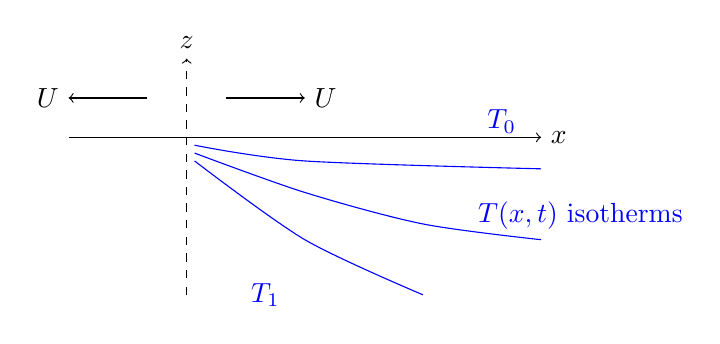
\begin{tikzpicture}
		\draw[->] (-3, 0) -- (3, 0) node[right] {$x$};
		\draw[dashed,->] (-1.5, -2) -- (-1.5, 1) node[above] {$z$};
		\draw[->] (-1, 0.5) -- (0, 0.5) node[right] {$U$};
		\draw[->] (-2, 0.5) -- (-3, 0.5) node[left] {$U$};
		\draw[smooth,blue] plot coordinates {(-1.4, -0.1) (0, -0.3) (3,
		-0.4)};
		\draw[smooth,blue] plot coordinates {(-1.4, -0.2) (0, -0.7) (1.5,
			-1.1) (3, -1.3)};
		\draw[smooth,blue] plot coordinates {(-1.4, -0.3) (0, -1.3) (1.5,
		-2)};
		\draw[blue] (3.5, -1) node {$T(x,t)$ isotherms};
		\draw[blue] (2.5, 0.2) node {$T_0$};
		\draw[blue] (-0.5, -2) node {$T_1$};
	\end{tikzpicture}
	\caption{Schematic diagram of mid-ocean ridge spreading and mantle
	temperature isotherms.}
\end{center}
\end{figure}


We wish to find the steady state profile with $\partial_t = 0, \symbf{u} = U
\hat{\symbf{x}}$ where $U$ is constant. Note that far from the ridge axis, the
thickness of the plate is much smaller than the extent of the plate. Hence in
terms of scalings, $z \ll x$ and we may neglect the $\partial_x^2$ component
of $\nabla^2$. We have
\begin{equation}
	U \frac{\partial T}{\partial x} = \kappa \left( \frac{\partial^2
	T}{\partial x^2} + \frac{\partial^2 T}{\partial z^2}\right) \approx \kappa
	\frac{\partial^2 T}{\partial z^2}
	\label{eq:temp}
\end{equation}
The scaling given by this equation is $U\Delta T / x \sim \kappa \Delta T /
z^2$ where $\Delta T = T_1 - T_0$ is the natural temperature scale. There is
no natural lengthscale, so we use that given by the advection-diffusion
equation:
\begin{equation}
	z \sim \sqrt{\frac{\kappa x}{U}}
\end{equation}

We can proceed by finding a self-similar solution with similarity variable
\begin{equation}
	\eta = \frac{z}{2\sqrt{\frac{\kappa x}{U}}}
\end{equation}
and seek solutions of the form
\begin{equation}
	\theta = \frac{T - T_0}{T_1-T_0} = \theta(\eta)
\end{equation}
Using the variables $\eta, \theta$, \eqref{eq:temp} becomes
\begin{align}
	-U\Delta T \frac{\eta}{2x} \theta_\eta &= \frac{\kappa \Delta T}{4
	\frac{\kappa x}{U}} \theta_{\eta\eta}\\
		\implies \theta_{\eta\eta} + 2\eta\theta_\eta &= 0
\end{align}
We can integrate directly to get $\theta_\eta = ae^{-\eta^2}$, which gives
\begin{equation}
	\theta = b + a \int_0^\eta e^{-y^2} \, \diffd y
\end{equation}
The boundary conditions are $\theta(0) = 1$ and $\theta(\infty) = 1$ based on
the definitions of $T_0$ and $T_1$. The thermal structure away from the ridge
is then
\begin{equation}
	T = T_0 + (T_1-T_0) \erf\left( \frac{z}{2\sqrt{\frac{\kappa x}{U}}}\right)
	\label{eq:T}
\end{equation}
where the error function $\erf$ and its complement erfc are defined by
\begin{align}
	\erf(x) &= \frac{2}{\sqrt{\pi}} \int_0^x e^{-y^2} \, \diffd y \\
	\text{erfc}(x) &= 1 - \erf(x)
\end{align}

\subsection{Ocean depth away from mid-ocean ridge}
We now consider the depth of the ocean following from the temperature field
derived above. We choose axes with $z$ increasing downwards, placing the sea
surface at $z=0$ and the `bottom' of the mantle at $z=H$. The coordinate $x$
increases away from the mid-ocean ridge, with ocean depth $w(x)$ at a given
$x$.

\begin{figure}
	\begin{center}
	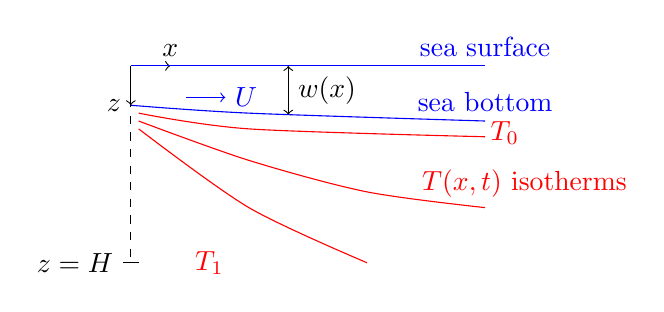
\begin{tikzpicture}
		\draw[->] (-1.5, 0.5) -- (-1.5, 0) node[left] {$z$};
		\draw[->] (-1.5, 0.5) -- (-1, 0.5) node[above] {$x$};
		\draw[dashed] (-1.5, 0.5) -- (-1.5, -2);

		\draw[blue,->] (-0.8, 0.1) -- (-0.3, 0.1) node[right] {$U$};
		\draw[blue] (-1.5, 0.5) -- (3, 0.5) node[above] {sea surface};

		\draw[smooth,red] plot coordinates {(-1.4, -0.1) (0, -0.3) (3,
		-0.4)};
		\draw[smooth,red] plot coordinates {(-1.4, -0.2) (0, -0.7) (1.5,
			-1.1) (3, -1.3)};
		\draw[smooth,red] plot coordinates {(-1.4, -0.3) (0, -1.3) (1.5,
		-2)};
		\draw[red] (3.5, -1) node {$T(x,t)$ isotherms};
		\draw[red] (3.25, -0.35) node {$T_0$};
		\draw[red] (-0.5, -2) node {$T_1$};

		\draw[smooth,blue] plot coordinates {(-1.5,0) (0, -0.1) (3, -0.2)};
		\draw[blue] (3, -0.2) node[above] {sea bottom};

		\draw[<->] (0.5, 0.5) -- (0.5, -0.12) node[midway,right] {$w(x)$};
		\draw (-1.4, -2) -- (-1.6, -2) node[left] {$z=H$};
	\end{tikzpicture}
	\caption{Schematic diagram of ocean depth and crust temperature surfaces.}
\end{center}
\end{figure}

First, consider \emph{isostacy}: Archimedean buoyancy applied
to Earth's crust. This indicates the depth at which an object/fluid parcel of some 
density lies in a fluid of different density. 
\begin{center}
	\begin{tikzpicture}[scale=2]
		\draw[blue] (-2, 0) -- (-1, 0); 
		\draw (-1, 0.3) -- (1, 0.3) -- (1, -0.3) -- (-1,
		-0.3) -- (-1, 0.3);
		\draw[blue] (1, 0) -- (2, 0);
		\draw[<->] (0.5, 0.3) -- (0.5, -0.3) node[midway,right] {$h$};
		\draw (-0.5, 0) node {$\rho_c$};
		\draw (-1.5, -0.3) node {$\rho_m$};
		\draw[<->] (1.2, 0) -- (1.2, -0.3) node[midway, right] {$b$};
	\end{tikzpicture}
\end{center}
Denoting the density of the crust and mantle as $\rho_c, \rho_m$ respectively,
the crust of thicknes $h$ sits at a depth $b$ in the mantle. Hydrostatic
balance gives $\rho_c g h = \rho_m g b$. Equivalently, we can consider a force
balance between the weight of the curst and the buoyancy force:
\begin{equation}
	\rho_c (h-b) g = (\rho_m - \rho_c) gb
\end{equation}

Within the oceanic lithosphere we have a denssity field
\begin{equation}
	\rho = \rho_m \left( 1- \alpha (T - T_1)\right)
\end{equation}
where $T=T(x,z)$ is the thermal model derived above, given by \eqref{eq:T}.
Isostatic balance gives the following, which balances water weight, mantle
weight, with water and mantle buoyancy. The ocean density is denoted by
$\rho_w$.

\begin{align}
	\rho_w w_0 + \rho_m (H - w_0) &= \rho_w w(x) + \int_w^H \rho(T) \, \diffd
	z \\
	  &= \rho_w w + \rho_m (H-w) - \rho_m \alpha \int_w^H (T-T_1) \, \diffd z \\
	\implies (\rho_m - \rho_w)(w-w_0) &= - \rho_m \alpha \int_w^H (T-T_1) \,
	\diffd z \\
	&\approx  - \rho_m \alpha (T_1 - T_0) \int_0^\infty \text{erfc}(\eta)
	\cdot 2 \sqrt{\frac{\kappa x}{U}} \, \diffd \eta
\end{align}
where the last approximate equality follows from taking $w \to 0$ and $H \to
\infty$, approximating the fact the mantle is much deeper than the ocean. The
ocean depth is therefore
\begin{equation}
	w-w_0 = \frac{\rho_m}{\rho_m - \rho_w} \alpha (T_1-T_0)
	\frac{2}{\sqrt{\pi}} \left(\frac{\kappa x}{U}\right)^{1/2}
\end{equation}
This model fits the data well near to the mid-ocean ridge, with crust age up
to 75 million years. However, away from the ridge, the model breaks down as
$w$ tends to a constant as $x \to \infty$. The breakdown of the model is due
to convection: the infinite depth curst approximation breaks down and
convection dynamics become important.

\section{Natural convection}
Natural convection arises in flows driven by density differences in a
gravitational field, e.g. due to temperature or composition.

\subsection{Static stability}
Consider the case of no fluid motion $\symbf{u} = 0$ and initial
stratification $\rho = \rho_0 (1+\beta z)$.  If $\beta < 0$, the dynamics are
statically stable. If $\beta > 0$, the dynamics are statically unstable but
dynamically could be stable. 

\begin{center}
	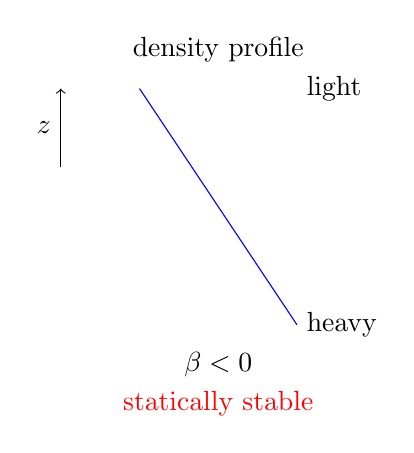
\begin{tikzpicture}
		\draw[blue] (0,0) -- (2, -3);
		\draw (2, 0) node[right] {light};
		\draw (2, -3) node[right] {heavy};

		\draw[->] (-1, -1) -- (-1, 0) node [midway,left] {$z$};
		\draw (1, -3.5) node {$\beta < 0$};
		\draw (1, 0.5) node {density profile};
		\draw[red] (1, -4) node {statically stable};
	\end{tikzpicture}
	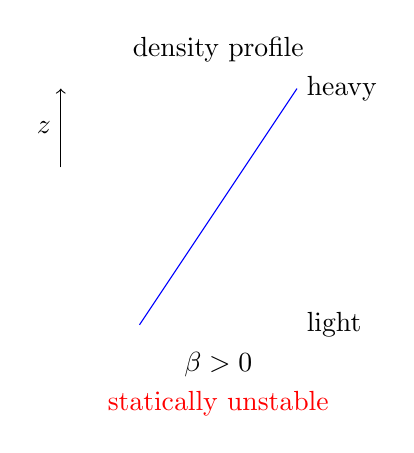
\begin{tikzpicture}
		\draw[blue] (2,0) -- (0, -3);
		\draw (2, -3) node[right] {light};
		\draw (2, 0) node[right] {heavy};

		\draw[->] (-1, -1) -- (-1, 0) node [midway,left] {$z$};
		\draw (1, -3.5) node {$\beta > 0$};
		\draw (1, 0.5) node {density profile};
		\draw[red] (1, -4) node {statically unstable};
	\end{tikzpicture}
\end{center}

\paragraph{Scaling analysis.} Consider a fluid parcel of characteristic size
$l$ in unstable density profile $\rho = \rho_0 (1+\beta z), \beta > 0$.
Suppose the parcel moves up a distance $h$ in time $\tau$.
\begin{center}
	\begin{tikzpicture}
		\draw[blue] (2,0) -- (0, -3);
		\draw (0.7, -3+0.7*3/2) circle (0.2);
		\draw[<->] (1, -2.15) -- (1, -1.75) node[midway,right] {$l$};
		\draw[dashed] (0.7, -1) circle (0.2);
		\draw[<->] (0.3, -3+0.7*3/2) -- (0.3, -1) node[midway,left] {$h$};
		\draw[blue] (2,0) node[right] {$\rho = \rho_0 (1+\beta z)$};
	\end{tikzpicture}
\end{center}

The rise of the fluid parcel relasess potential energy $E$ which scales as
\begin{equation}
	E \sim (\Delta \rho l^3) g h \sim (\rho_0 \beta h l^3) g h \sim \rho_0
	\beta g h^2 l^3
\end{equation}
The timescale for the rise is limited by diffusion buoyancy $\tau \sim
l^2/\kappa$ where $\kappa$ is thermal diffusivity. Viscous dissipation over
timescale $\tau$ scales as the shear stress times the distance travelled:
\begin{equation}
	\mathcal{D} \sim \frac{\mu U}{l}l^2 h \sim \mu \frac{h/\tau}{l} l^2 h \sim
	\frac{\mu \kappa h^2}{l}
\end{equation}

Instability arises if $E \gtrapprox \mathcal{D}$, which we can write as
\begin{equation}
	\rho_0 \beta g h^2 l^3 \gtrapprox \frac{\mu \kappa h^2}{l}
\end{equation}
Define the \emph{Rayleigh number}
\begin{equation}
	\text{Ra} = \frac{\rho_0 \beta g l^4}{\kappa \mu}
\end{equation}
Then there is instability if $\text{Ra} \gtrapprox \mathcal{O}(1)$.

\subsection{Onset of convection}
Consider a fluid of depth $h$ between $z=0$ and $z=h$ with density profile
$\rho(z)$ and temperature difference $\Delta T$ across the depth.

\begin{center}
	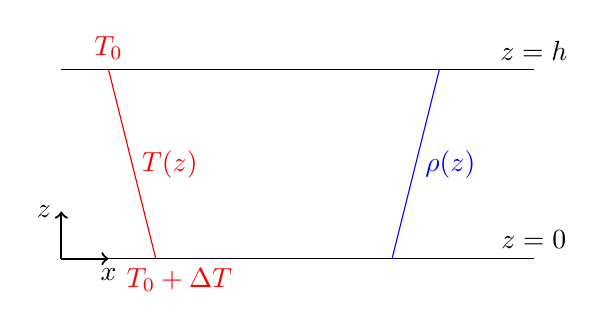
\begin{tikzpicture}[scale=1.2]
		\draw  (0, 2) -- (5, 2);
		\draw (0, 0) -- (5, 0);
		\draw[thick,->] (0, 0) -- (0.5, 0) node[below] {$x$};
		\draw[thick,->] (0, 0) -- (0, 0.5) node[left] {$z$};
		\draw (5, 0.2) node {$z=0$};
		\draw (5, 2.2) node {$z=h$};
		\draw[red] (0.5, 2) -- (1, 0) node[midway,right] {$T(z)$};
		\draw[red] (0.5, 2) node[above] {$T_0$};
		\draw[red] (1.25, 0) node[below] {$T_0 + \Delta T$};
		\draw[blue] (3.5,0) -- (4, 2) node[midway,right] {$\rho(z)$};
	\end{tikzpicture}
\end{center}

The governing equations are conservation of mass \eqref{eq:masscons},
conservation of momentum \eqref{eq:momcons}, and conservation of energy
\eqref{eq:energycons}.
\begin{align}
	\nabla \cdot \symbf{u} &= 0 \label{eq:masscons} \\
	\rho \left( \frac{\partial \symbf{u}}{\partial t} +
	\symbf{u}\cdot\nabla\symbf{u}\right) &= - \nabla p + \mu \nabla^2
	\symbf{u} - \rho g \hat{\symbf{z}} \label{eq:momcons} \\
	\rho c_p \left( \frac{\partial T}{\partial t} + \symbf{u} \cdot \nabla T
	\right) &= \nabla \cdot (k \nabla T) \label{eq:energycons}
\end{align}

For steady solutions with $\symbf{u} = 0$ and $\partial_t = 0$ we find
\begin{align}
	T &= T_0 + \Delta T \left(1-\frac{z}{h}\right) \\
	\frac{\partial p}{\partial x} = \frac{\partial p}{\partial y} &= 0 \\
	\frac{\partial p}{\partial z} &= - \rho_0 g \left( 1- \alpha
	(T-T_0)\right) 
\end{align}
We assess the stability by examining small perturbations to a steady base
state:
\begin{align}
	\symbf{u} &= 0 + \symbf{u}'(\symbf{x},t) \\
	T &= T_0 + \Delta T \left(1-\frac{z}{h}\right) + T'(\symbf{x},t) \\
	p &= p_0(z) + p'(\symbf{x},t) 
\end{align}
The linearied perturbation equations are thus
\begin{align}
	\nabla \cdot \symbf{u}' &= 0  \\
	\rho_0  \frac{\partial \symbf{u}'}{\partial t} &= - \nabla p' + \mu
	\nabla^2 \symbf{u}' + \rho_0 g \alpha T' \hat{\symbf{z}} \\
	\frac{\partial T'}{\partial t} - \frac{\Delta T}{h} w' &= \kappa \nabla^2
	T'
\end{align}

We wish to non-dimensionalise these equations. There are two intrinsic
scales, temperature $\sim \Delta T$ and lengths $\sim h$. We form velocity and
time characteristic scales via \emph{diffusive scaling}. From the thermal
equation:
\begin{equation}
	\frac{\Delta T}{t} \sim \frac{\Delta T U}{h} \sim \frac{\kappa \Delta
	T}{h^2}
\end{equation}
From the second relation we have $U \sim \kappa/h$, then from the first we
have $t \sim h^2/\kappa$.  The non-dimensionalised equations (dropping $'$
henceforth) are
\begin{align}
	\nabla \cdot \symbf{u} &= 0 \\
	\frac{1}{\text{Pr}} \frac{\partial \symbf{u}}{\partial t} &= - \nabla p +
	\nabla^2 \symbf{u} + \text{Ra}T \hat{\symbf{z}} \\
	\frac{\partial T}{\partial  t} - w &= \nabla^2 T 
\end{align}
where the \emph{Prandtl number} $\text{Pr} = \frac{\mu/\rho_0}{\kappa}$ which
quantifies the importance of viscous diffusion versus thermal diffusion.


\end{document}
